%%%%%%%%%%%%%%%%%%%%%%%%%%%%%%%%%%%%%%%%%%%%%%%%%%%%%%%%%%%%%%%%%%%%%%%%%%%%%%%%
%2345678901234567890123456789012345678901234567890123456789012345678901234567890
%        1         2         3         4         5         6         7         8

\documentclass[letterpaper, 10 pt, conference]{ieeeconf}

\IEEEoverridecommandlockouts
\overrideIEEEmargins

\usepackage{cite}
\usepackage{amsmath,amssymb,amsfonts}
\usepackage{algorithmic}
\usepackage{graphicx}
\usepackage{textcomp}
\usepackage{xcolor}
\usepackage{float}
\usepackage{multirow}

\graphicspath{{../IJCNN/}}

\def\BibTeX{{\rm B\kern-.05em{\sc i\kern-.025em b}\kern-.08em
    T\kern-.1667em\lower.7ex\hbox{E}\kern-.125emX}}

% -----------------------------------------------------------------------

\title{\LARGE \bf
Layer-Wise Attribute Sensitivity and Adaptive Fusion with Mixture of
Experts in Deep Models for Color and Texture Classification
}

\author{
    Arlete T. Beuren\textsuperscript{1},
    Vinícius C. Ribeiro\textsuperscript{1},
    Leonardo J. R. Pinto\textsuperscript{1},
    Jonathan de Matos\textsuperscript{2},
    Alceu S. Britto Jr.\textsuperscript{2,3}%
    \thanks{This work was supported by the Conselho Nacional de
            Desenvolvimento Cient\'{i}fico e Tecnol\'{o}gico (CNPq, Brazil).}%
    \thanks{\textsuperscript{1}Universidade Tecnol\'{o}gica Federal do
            Paran\'{a} (UTFPR), Santa Helena (PR), Brazil.
            \texttt{arletebeuren@utfpr.edu.br}}%
    \thanks{\textsuperscript{2}Universidade Estadual de Ponta Grossa (UEPG),
            Ponta Grossa (PR), Brazil.
            \texttt{jonathan@uepg.br}}%
    \thanks{\textsuperscript{3}Pontif\'{i}cia Universidade Cat\'{o}lica do
            Paran\'{a} (PUCPR), Curitiba (PR), Brazil.
            \texttt{alceu@ppgia.pucpr.br}}%
}

% -----------------------------------------------------------------------

\begin{document}

\maketitle
\thispagestyle{empty}
\pagestyle{empty}

% -----------------------------------------------------------------------
\begin{abstract}

This study addresses the challenge of effectively extracting image content
based on specific visual attributes — color, texture, or their combination
— and proposes an adaptive fusion strategy based on Mixture of
Experts~(MoE).
Experiments are conducted with five architectures — ResNet-50, VGG-16,
iBOT, VMamba, and LMFCN — on a fashion dataset comprising 1,000 color
images and 1,000 texture images.
\emph{Experiment~1} confirms that early layers are more effective for
color classification, while deeper layers excel at texture recognition,
a pattern that generalizes from classical CNNs to Vision Transformers and
State Space Models.
\emph{Experiment~2} shows that simple concatenation of early and deep
layer features generally does not outperform specialized single-layer
representations.
\emph{Experiment~3} introduces a trainable MoE model that, through a
learned router, adaptively weights the contributions of the early
(color-sensitive) and deep (texture-sensitive) layers on a per-image
basis.
The MoE outperforms both Experiment~1 and Experiment~2 in nearly all
architectures, achieving up to 98.00\% with VMamba on texture and 97.33\%
with iBOT on color — improvements of 2.24 and 1.46 percentage points over
the best individual layers, respectively.

\end{abstract}

\begin{IEEEkeywords}
Convolutional Neural Networks, Deep Models, Visual Attributes, Vision
Transformers, State Space Models, Mixture of Experts, Image Retrieval.
\end{IEEEkeywords}

% -----------------------------------------------------------------------
\section{INTRODUCTION}

Advances in convolutional neural networks (CNNs) have enabled increasingly
effective computer vision solutions for industrial applications.
A prominent example is image retrieval in e-commerce, where search queries
can be performed using text, images, or multimodal
combinations~\cite{b1}.

Image content-based retrieval systems present unique challenges and have
applications beyond e-commerce, including medical imaging, geographic
information systems, and surveillance~\cite{b12}.
A key challenge lies in accurately extracting relevant visual attributes
from images, particularly when user queries are driven by specific
properties such as color, texture, or their combination
(Figure~\ref{fig_patterns}).

\begin{figure}[htbp]
\centerline{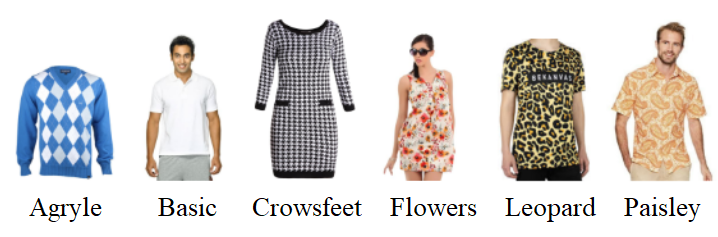
\includegraphics[width=0.48\textwidth]{fig_texture_samples.png}}
\caption{Six different color and texture-based patterns
         (adapted from~\cite{b2}).}
\label{fig_patterns}
\end{figure}

Color and texture feature extraction has been a central topic in
Content-Based Image Retrieval (CBIR).
Classical color descriptors include color histograms and color moments,
which capture statistical properties such as mean, variance, and skewness
of color distributions~\cite{b24}.
For texture representation, methods such as Gabor filters and Local Binary
Patterns (LBP) have been widely used~\cite{b25}.

With the advent of deep learning, Baloian et al.~\cite{b2} demonstrated
that different CNN layers exhibit attribute-specific sensitivity, with
early layers being more responsive to color information and deeper layers
capturing texture patterns.
However, the behavior of attribute-specific representations across modern
architectures — Vision Transformers and State Space Models — remains
underexplored, and adaptive fusion strategies between specialized layers
are still scarce in the literature.

In this work, we evaluate and compare classical and modern deep
architectures for color- and texture-based image classification.
We analyze layer-wise representations to investigate their sensitivity to
visual attributes and the effectiveness of different fusion strategies.
As a main contribution, we propose an adaptive fusion model based on
Mixture of Experts~(MoE) that learns, on a per-image basis, the relative
weights of the early (color) and deep (texture) layers through a trainable
router.

The dataset used was introduced in~\cite{b2} and consists of fashion
images including hats, dresses, shirts, socks, purses, and scarves.
It is divided into two subsets:
\begin{itemize}
  \item \textbf{Color dataset}: 1,000 images across 10 color classes
        (red, black, blue, green, yellow, gray, brown, pink, purple, and
        orange), illustrated in Figure~\ref{fig_color_samples};
  \item \textbf{Texture dataset}: 1,000 images across 10 texture pattern
        classes (squared, striped, flowers, leopard, polka dots, basic,
        paisley, argyle, crowsfeet, and sequin).
\end{itemize}

\begin{figure}[htbp]
\centerline{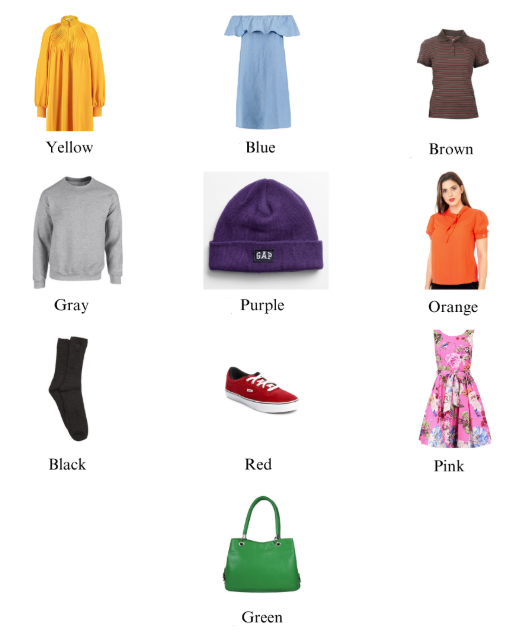
\includegraphics[width=0.48\textwidth]{fig_color_samples.png}}
\caption{Sample images from each class in the color dataset.}
\label{fig_color_samples}
\end{figure}

The main contributions of this work are:
\begin{itemize}
  \item A comprehensive layer-wise analysis of attribute sensitivity across
        classical CNNs, Vision Transformers, and State Space Models;
  \item A comparative benchmark of VGG-16, ResNet-50, iBOT, VMamba, and
        LMFCN for color- and texture-based image classification;
  \item Experimental demonstration that simple concatenation fusion does
        not improve performance for attribute-specific tasks;
  \item Proposal and evaluation of an MoE model that performs adaptive
        fusion of early and deep layer features, outperforming both
        concatenation and single-layer representations in most settings.
\end{itemize}

This paper is organized as follows.
Section~II reviews related work.
Section~III describes the evaluated backbone architectures.
Section~IV details the experimental methodology.
Section~V presents the results.
Section~VI discusses the findings, and Section~VII concludes the paper.

% -----------------------------------------------------------------------
\section{RELATED WORK}

The use of convolutional neural networks for representing object similarity
has been extensively explored.
Baloian et al.~\cite{b2} investigated the behavior of ResNet-50 layers for
color and texture-based retrieval, showing that early convolutional layers
are more sensitive to color, while deeper layers better capture texture
patterns.
Features were extracted from ResNet-50 pre-trained on
ImageNet~\cite{b3}, with Global Average Pooling (GAP) applied to each
residual block and k-nearest neighbors (kNN) used for classification with
5 repetitions of stratified 70/30 holdout.

The hierarchical nature of representations in deep networks has been
investigated since the seminal work of Zeiler and
Fergus~\cite{bzeiler}, who showed visually that early CNN layers respond
to edges and colors while deeper layers encode complex structural patterns.
Analogous analyses for Vision Transformers were conducted by
Kazami et al.~\cite{bkazami}, revealing that early ViT blocks preserve
low-level spatial information while final blocks capture global semantics.
In contrast to these works, which perform qualitative or visualization-based
analyses, the present study conducts a systematic quantitative evaluation
of layer-wise sensitivity to specific visual attributes (color and
texture), extends the analysis to State Space Model architectures (VMamba)
not yet covered in the layer-analysis literature, and proposes a trainable
adaptive fusion mechanism grounded in these findings.

Several studies have explored representation learning for object and
attribute recognition.
Liang et al.~\cite{b10} employed neural networks to learn discriminative
features based on object categories, while Gan et al.~\cite{b11} proposed
multi-source domain generalization techniques for cross-domain attribute
learning.
Siamese architectures have been investigated for fine-grained
classification; Moresco et al.~\cite{b8} demonstrated that combining
intermediate-layer features improves plant species classification,
highlighting the complementary nature of multi-layer representations.

Classical texture and color descriptors remain relevant for CBIR systems.
Irtaza et al.~\cite{b13} proposed a texture extraction framework based on
wavelet packets and Gabor filter eigenvalues.
Lin et al.~\cite{b15} introduced color co-occurrence matrices (CCM),
difference between pixels of scan patterns (DBPSP), and color
histogram-based clustering (CHKM).

Multi-layer feature fusion has been proposed to combine representations
from different network depths.
Strategies include early fusion (feature concatenation), late fusion
(decision-level combination), and learned fusion using attention
mechanisms~\cite{b26,b27}.
However, the effectiveness of such approaches for attribute-specific tasks
remains insufficiently studied.

Recent advances have challenged the dominance of Transformer-based models.
The Mamba architecture~\cite{b16} is a Structured State Space Model (SSM)
achieving linear time complexity, and the iBOT
framework~\cite{b17} introduced masked image modeling with an online
tokenizer for self-supervised visual representation learning.
The LMFCN framework~\cite{b28} trains Fully Convolutional Networks whose
representations are optimized for large-margin classification using SVMs.

Mixture of Experts~(MoE) was originally proposed by
Jacobs et al.~\cite{bmoe_orig} as a modular architecture in which a router
learns to divide the input space among local experts.
Recent work explores MoE for multimodal image fusion: Cao
et al.~\cite{bmoe_cao} proposed MoE-Fusion, combining local and global
experts through a multi-modal gated router for dynamic image fusion.
However, the application of MoE to adaptive depth-wise layer selection
within a single backbone for specific visual attributes remains unexplored.
This work addresses this gap by proposing a trainable router that learns,
per image, how much to weight the early-layer (color) versus deep-layer
(texture) representation.

% -----------------------------------------------------------------------
\section{EVALUATED BACKBONE MODELS}

This section describes the five backbone architectures used in the
experiments.

\subsection{ResNet-50}

ResNet-50~\cite{b4} is a 50-layer CNN that employs residual learning via
identity-based skip connections, mitigating gradient degradation and
enabling stable training at large depths.
In Experiment~1, features are extracted from each residual block via GAP
(dimensions: 256, 512, 1024, and 2048).
In the MoE model, the early layer corresponds to Residual Block~1~(256d)
and the deep layer to Residual Block~3~(1024d)
(Figure~\ref{fig_resnet}).

\begin{figure}[htbp]
\centerline{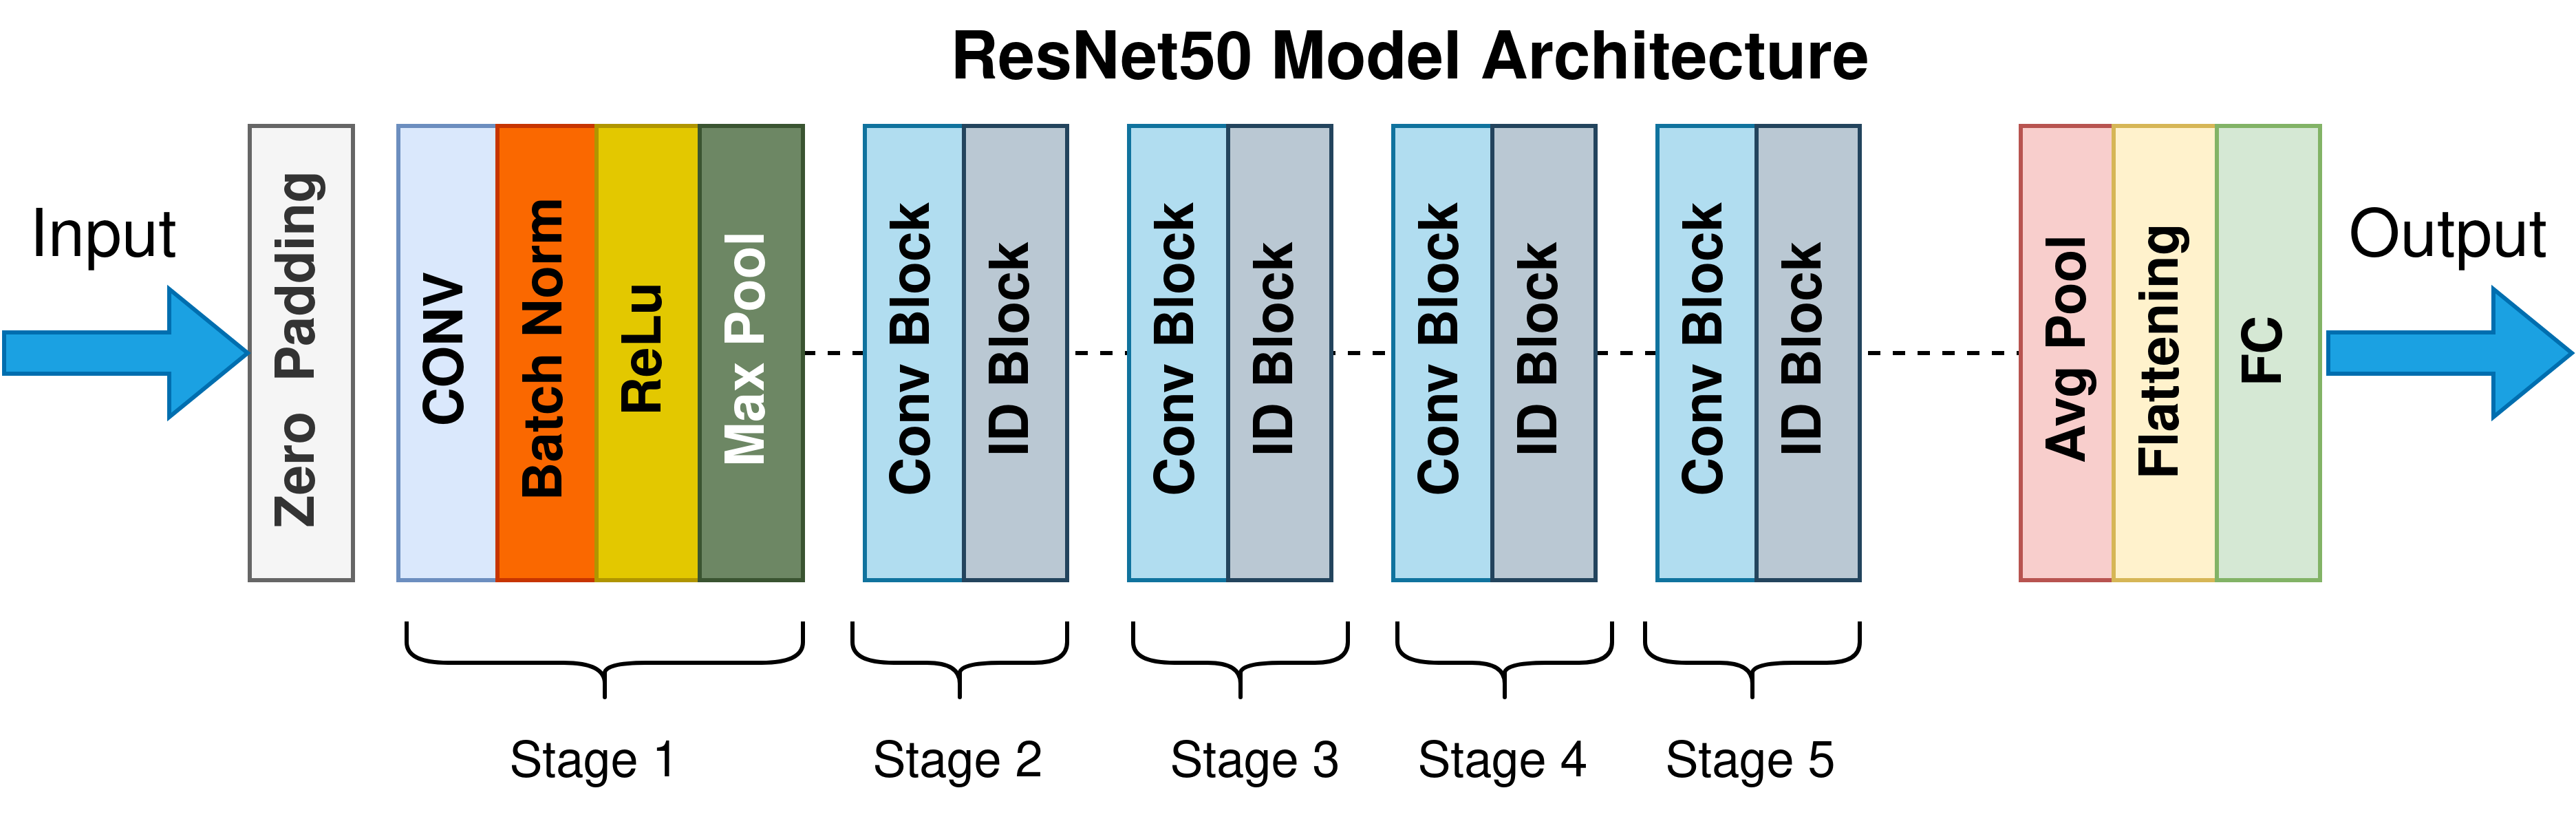
\includegraphics[width=0.48\textwidth]{resnet50.png}}
\caption{ResNet-50 architecture. Adapted from Mukherjee~\cite{b23},
         based on He et al.~\cite{b4}.}
\label{fig_resnet}
\end{figure}

\subsection{VGG-16}

VGG-16~\cite{b7} employs a homogeneous architecture with stacked
$3 \times 3$ convolutional layers across 5 convolutional blocks with
output dimensions 64, 128, 256, 512, and 512.
In the MoE model, the early layer corresponds to Block~1~(64d) and the
deep layer to Block~3~(256d) (Figure~\ref{fig_vgg}).

\begin{figure}[htbp]
\centerline{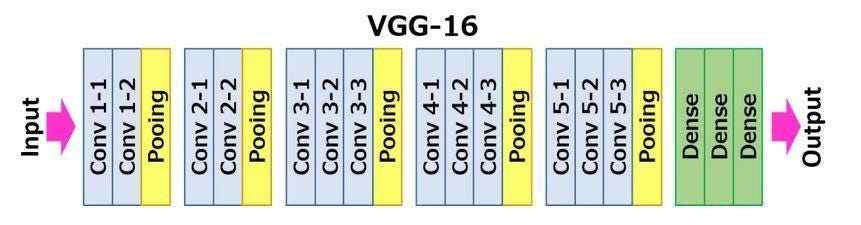
\includegraphics[width=0.48\textwidth]{VGG16.jpg}}
\caption{VGG-16 architecture.
         Source: Simonyan \& Zisserman~\cite{b7}.}
\label{fig_vgg}
\end{figure}

\subsection{VMamba}

VMamba~\cite{b16} is a Structured State Space Model (SSM) that processes
sequences in linear time via a selective scanning mechanism.
We use the VMamba-Tiny variant; features are extracted from each of its
four stages via GAP (dimensions: 96, 192, 384, and 768).
In the MoE, the early layer is Stage~1~(192d) and the deep layer is
Stage~2~(384d) (Figure~\ref{fig_mamba}).

\begin{figure}[htbp]
\centerline{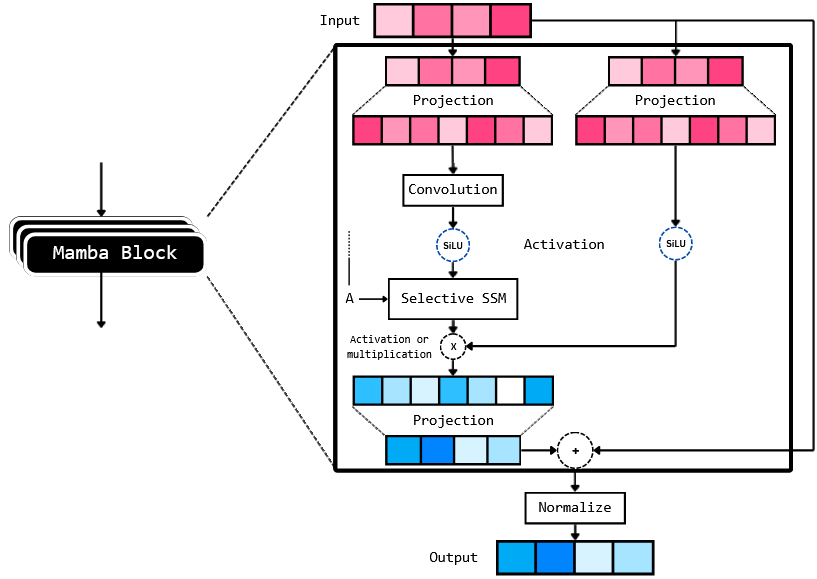
\includegraphics[width=0.48\textwidth]{Vmamba.png}}
\caption{Mamba block diagram.
         Source: Gu \& Dao~\cite{b16}.}
\label{fig_mamba}
\end{figure}

\subsection{iBOT}

iBOT~\cite{b17} is a self-supervised framework based on Vision
Transformers (ViT) using masked image modeling with an online tokenizer.
We use the ViT-S/16 backbone; features are extracted from each of its
12 transformer blocks via the CLS token (384 dimensions each).
In the MoE, the early layer is Block~2 and the deep layer is Block~9
(Figure~\ref{fig_ibot}).

\begin{figure}[htbp]
\centerline{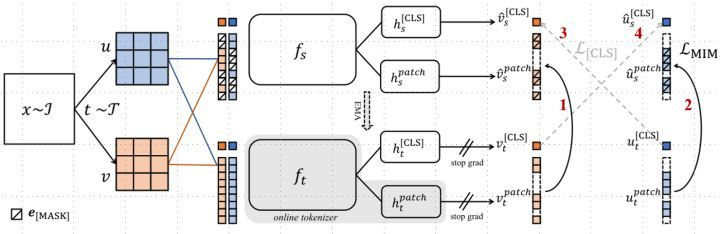
\includegraphics[width=0.48\textwidth]{Ibot.jpg}}
\caption{iBOT framework overview.
         Source: Zhou et al.~\cite{b17}.}
\label{fig_ibot}
\end{figure}

\subsection{LMFCN}

The LMFCN~\cite{b28} framework trains Fully Convolutional Networks (FCNs)
whose learned representations are optimized for large-margin SVM
classification.
We evaluate TCNN architectures (3 to 6 layers) trained from scratch and
pre-trained ResNet-18 variants with the final layers removed
(Figure~\ref{fig_lmfcn}).
Because LMFCN relies on an external SVM classifier tightly coupled to the
FCN training objective, integrating a trainable MoE router into its
framework would require non-trivial architectural modifications; LMFCN is
therefore evaluated under Experiments~1 and~2 only.

\begin{figure}[htbp]
\centerline{\includegraphics[width=0.48\textwidth]{CNNSV4.eps}}
\caption{LMFCN overview.
         Source: de Matos et al.~\cite{b28}.}
\label{fig_lmfcn}
\end{figure}

% -----------------------------------------------------------------------
\section{EXPERIMENTAL METHODOLOGY}

\subsection{Dataset and Protocol}

The dataset was introduced in~\cite{b2} and consists of 10 color classes
and 10 texture classes with 100 images per class, totaling 1,000 images
per task.
Data were split into 70\% training and 30\% test across 5 repetitions of
stratified holdout.
Following the protocol established in~\cite{b2} and widely adopted in the
attribute-based CBIR literature, feature vectors are evaluated with a
k-nearest neighbor (kNN) classifier ($k=5$, Euclidean distance).

\subsection{Layer-Wise Sensitivity Analysis}

For each architecture, features are extracted from each individual layer
or processing block.
CNNs use GAP to produce a single feature vector per layer; iBOT uses the
CLS token; VMamba applies GAP to each stage's feature map.
For LMFCN, we evaluate TCNN variants (3–6 layers) and ResNet-18 with 2 or
4 residual blocks.

\subsection{Early--Deep Concatenation Fusion}

For each backbone, features from the best color layer~(E) and the best
texture layer~(D) are concatenated: $z = [f_E \; ; \; f_D]$, and the
resulting vector is evaluated with kNN.

\subsection{Adaptive Fusion with Mixture of Experts}

The proposed MoE model learns, per image, adaptive weights $\alpha$ and
$\beta$ for the early and deep layers, respectively.

\textbf{Architecture.} For each backbone, two projection heads $h_E$ and
$h_D$ — each comprising a linear layer, LayerNorm, and ReLU — map
heterogeneous-dimensional features to a common space of dimension $d=256$.
A Router (two-layer MLP with Softmax) receives the concatenation
$[h_E(f_E) ; h_D(f_D)]$ and produces weights $\alpha$ and $\beta$ with
$\alpha + \beta = 1$.
The final embedding is:
\begin{equation}
    z = \alpha \cdot h_E(f_E) + \beta \cdot h_D(f_D).
    \label{eq:moe}
\end{equation}

The backbone is frozen during training; only $h_E$, $h_D$, and the Router
are updated.
An auxiliary linear head supervises training with cross-entropy loss; at
evaluation time, only the embeddings $z$ are used with kNN.

\textbf{Training protocol.}
AdamW optimizer, $lr = 10^{-4}$, weight decay $= 10^{-5}$,
CosineAnnealingLR with $T_{\max} = 30$ epochs, batch size 32, basic data
augmentation (random 224$\times$224 crop and horizontal flip) during
training only.
Final evaluation: kNN with $k=5$ and StandardScaler on embeddings $z$,
under the same 5-repetition holdout protocol.

Table~\ref{tab_moe_config} summarizes the early and deep layer selections
per backbone in the MoE model.

\begin{table}[htbp]
\caption{Early and deep layer configuration for each backbone in the MoE
         model.}
\begin{center}
\begin{tabular}{c|c|c|c|c}
\hline
\textbf{Backbone} & \textbf{Early (E)} & \textbf{Dim~E}
                  & \textbf{Deep (D)} & \textbf{Dim~D} \\
\hline
VGG-16    & Block 1     & 64   & Block 3     & 256  \\
ResNet-50 & Res. Block 1 & 256  & Res. Block 3 & 1024 \\
iBOT      & Block 2     & 384  & Block 9     & 384  \\
VMamba    & Stage 1     & 192  & Stage 2     & 384  \\
\hline
\end{tabular}
\label{tab_moe_config}
\end{center}
\end{table}

% -----------------------------------------------------------------------
\section{EXPERIMENTAL RESULTS}

The results are organized in two parts.
The first part~(Sections~V-A and~V-B) analyzes the layer-wise behavior
of each backbone's embeddings with respect to color and texture, using
kNN accuracy as a proxy for embedding discriminability.
The goal here is not to optimize classification, but to characterize
which layers best capture each visual attribute.
The second part~(Sections~V-C to~V-E) evaluates fusion strategies and,
finally, assesses the same embeddings under a CBIR protocol using
mAP@10, R@1, and R@5.

\subsection{Layer-Wise Sensitivity}

Table~\ref{tab_best_layer} summarizes the best layer per backbone for
color and texture classification.
Across all architectures, early layers consistently achieve higher color
accuracy, while deeper layers are more effective for texture — confirming
and extending the pattern originally reported for ResNet-50
in~\cite{b2}.
In VGG-16, Layer~1 peaks at 95.13\% for color, while Layer~4 reaches
94.73\% for texture.
ResNet-50 follows the same trend: Residual Block~2 for color~(95.87\%)
and Block~3 for texture~(93.27\%).
iBOT shows the steepest gradient across its 12 transformer blocks —
color accuracy falls from 94.53\% at Block~0 to 62.80\% at Block~11,
while texture climbs to 97.20\% at Block~9, the highest value among all
evaluated architectures.
VMamba exhibits a more compressed version of the same pattern across its
four stages, with Stage~1 best for color~(94.41\%) and Stage~2 for
texture~(95.76\%).

\begin{table}[htbp]
\caption{Best layer per backbone for color and texture classification
         (\%). Bold: highest value per attribute column.}
\begin{center}
\begin{tabular}{c|c|c|c|c|c|c}
\hline
\textbf{Backbone} & \textbf{Best Color} & \textbf{Color} & \textbf{Std}
                  & \textbf{Best Tex.}  & \textbf{Tex.}  & \textbf{Std} \\
\hline
VGG-16    & Layer 1 & 95.13          & 0.81 & Layer 4 & 94.73          & 0.74 \\
ResNet-50 & RB 2    & \textbf{95.87} & 0.50 & RB 3    & 93.27          & 0.25 \\
iBOT      & Block 2 & \textbf{95.87} & 1.05 & Block 9 & \textbf{97.20} & 0.54 \\
VMamba    & Stage 1 & 94.41          & 0.52 & Stage 2 & 95.76          & 0.84 \\
\hline
\end{tabular}
\label{tab_best_layer}
\end{center}
\end{table}

Figure~\ref{fig_depth} illustrates the full depth-accuracy curves,
showing the inverse pattern between color and texture for each backbone.

\begin{figure}[htbp]
\centerline{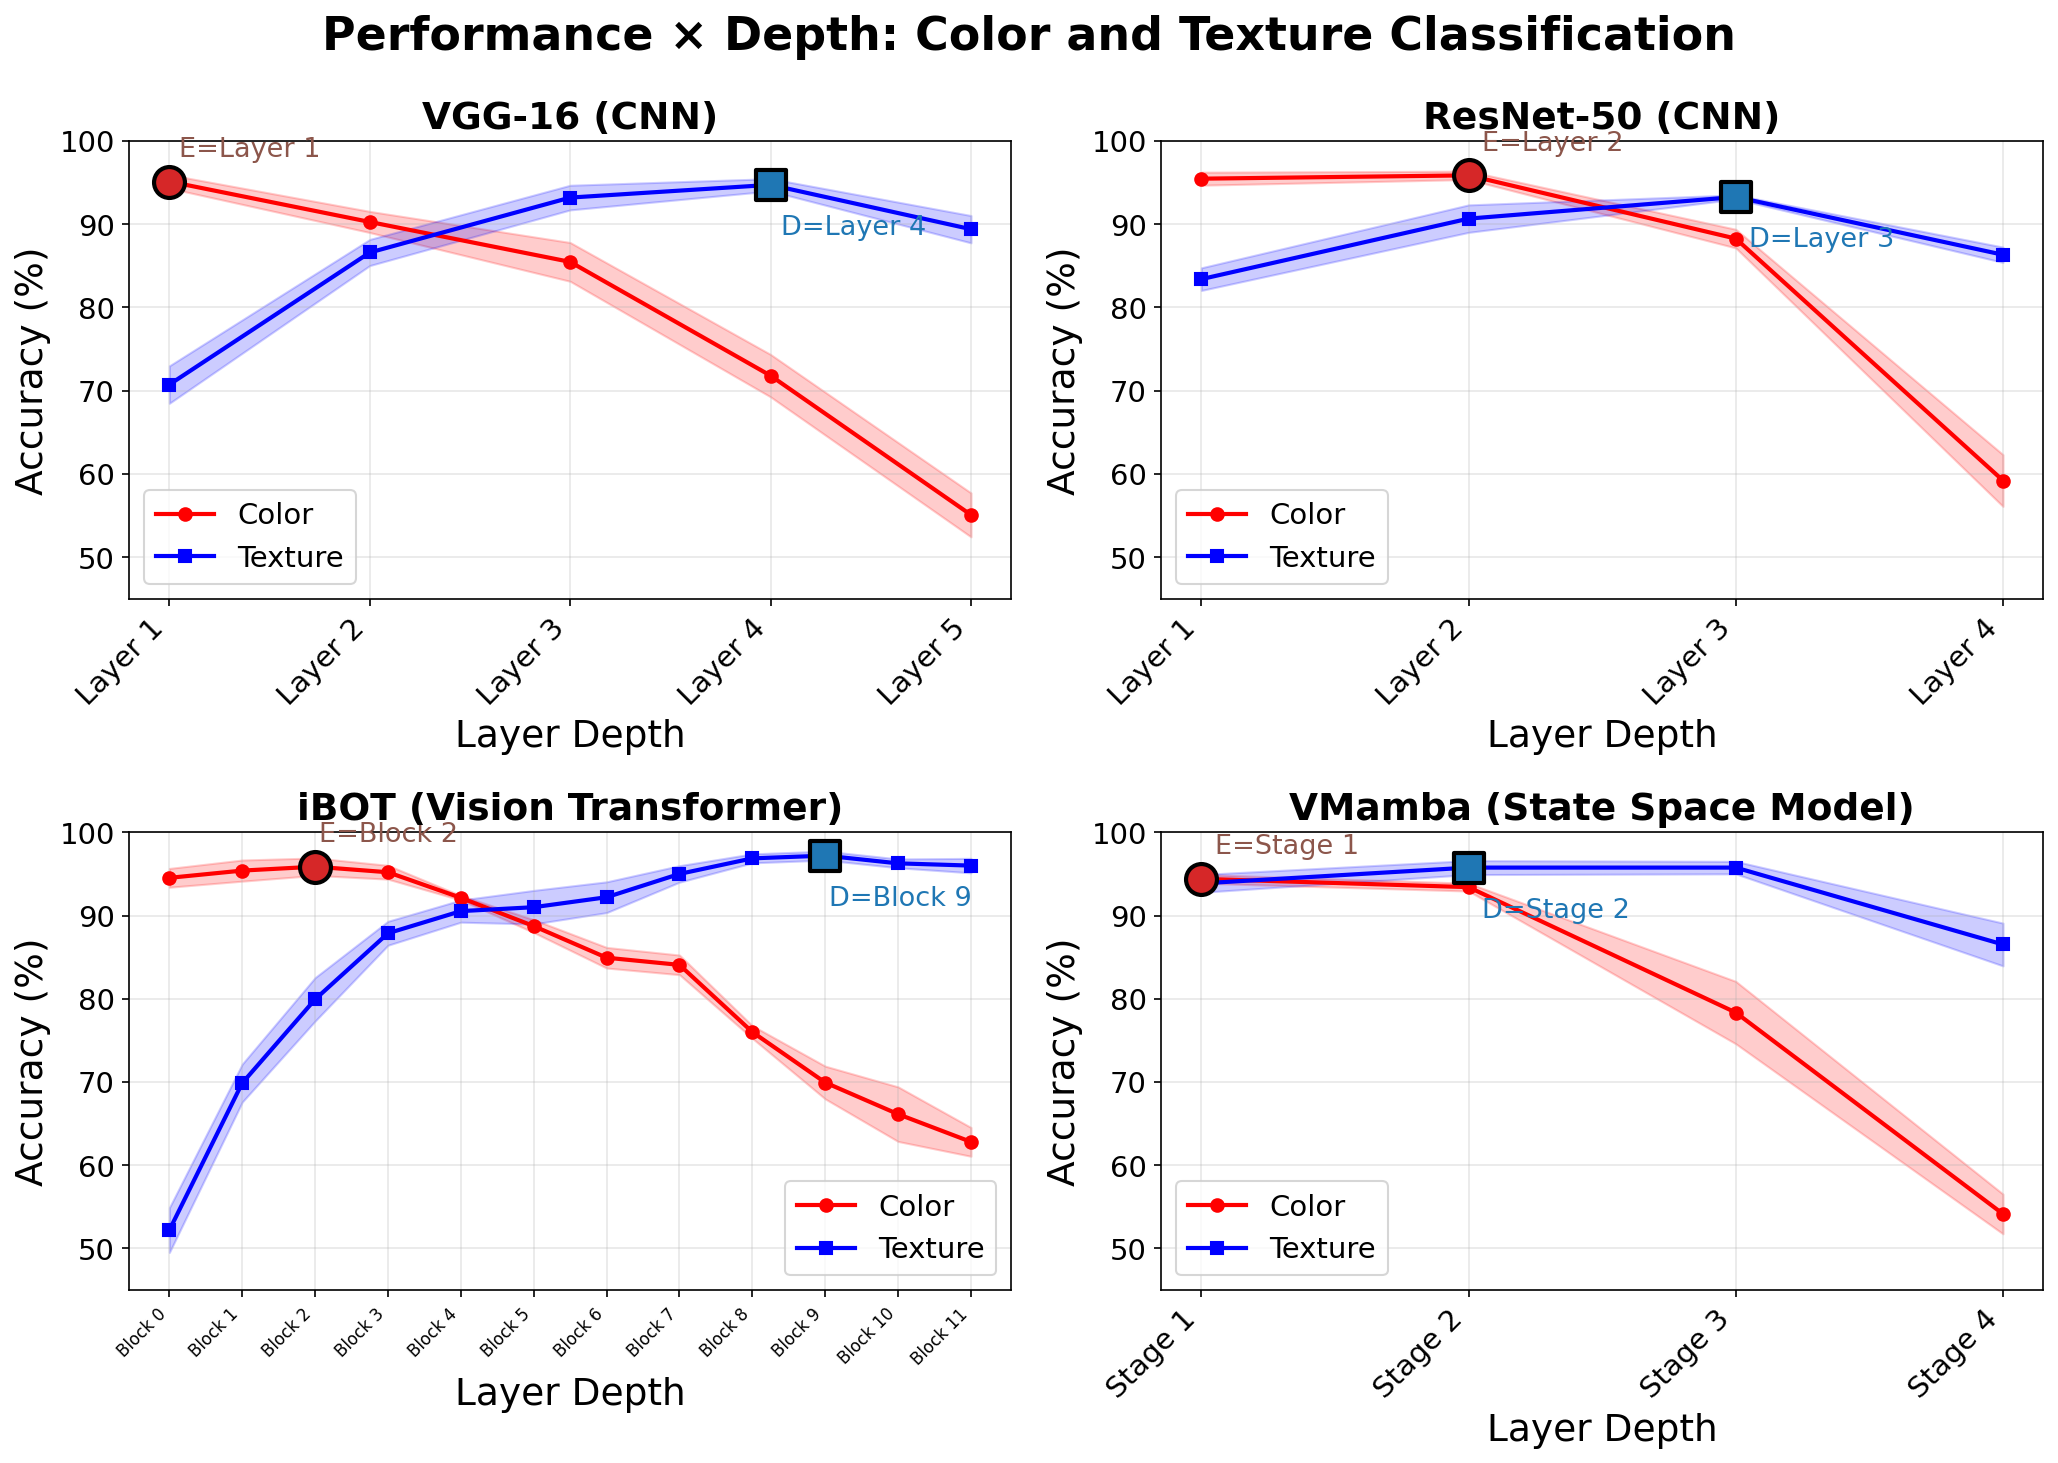
\includegraphics[width=0.48\textwidth]{curvas_desempenho_profundidade.png}}
\caption{Performance vs. depth: color and texture classification for
         VGG-16, ResNet-50, iBOT, and VMamba. Markers indicate the best
         layer per attribute (E=color, D=texture).}
\label{fig_depth}
\end{figure}

\subsection{Layer-Wise Sensitivity --- LMFCN}

Table~\ref{tab1} presents LMFCN results.
On the texture dataset, increasing TCNN depth consistently improves
performance.
On the color dataset, higher accuracy is obtained from earlier layers.
LMFCN with its SVM classifier achieved 96.87\%$\pm$0.9 on texture
(ResNet-18 with 2 blocks) and 97.73\%$\pm$0.95 on color (TCNN3).

\begin{table}[htbp]
\caption{Accuracy of ResNet-18 Convolutional Block (CB) and Residual
         Blocks (RB) and TCNN layers using LMFCN.}
\begin{center}
\begin{tabular}{c|c|c|c|c|c}
\hline
\textbf{Method} & \textbf{Color} & \textbf{Std}
                & \textbf{Tex.} & \textbf{Std} & \textbf{Dim} \\
\hline
TCNN3 Layer 3 & \textbf{95.94} & 0.43 & \textbf{58.27} & 1.30 & 640  \\
TCNN4 Layer 4 & \textbf{94.80} & 0.65 & \textbf{60.40} & 2.60 & 640  \\
TCNN5 Layer 5 & 95.40 & 0.96 & \textbf{62.93} & 1.65 & 640  \\
TCNN6 Layer 6 & 94.53 & 0.84 & \textbf{64.34} & 2.69 & 640  \\
ResNet-18(2) RB1 & \textbf{96.13} & 0.73 & 84.87 & 1.38 & 640  \\
ResNet-18(2) RB2 & 91.93 & 0.98 & \textbf{91.00} & 1.62 & 1280 \\
ResNet-18(4) RB1 & \textbf{95.93} & 0.98 & 84.13 & 1.59 & 640  \\
ResNet-18(4) RB3 & 89.53 & 1.37 & \textbf{92.47} & 1.48 & 2560 \\
\hline
\end{tabular}
\label{tab1}
\end{center}
\end{table}

\subsection{Results of Early--Deep Concatenation Fusion}

Table~\ref{tab5} shows the fusion configuration per backbone, and
Tables~\ref{tab6} and~\ref{tab7} present the results.

\begin{table}[htbp]
\caption{Fusion configuration for each backbone.}
\begin{center}
\begin{tabular}{c|c|c|c|c|c}
\hline
\textbf{Backbone} & \textbf{E (color)} & \textbf{Dim E}
                  & \textbf{D (tex.)} & \textbf{Dim D} & \textbf{Dim z} \\
\hline
VGG-16    & Layer 1 & 64  & Layer 4 & 512  & 576  \\
ResNet-50 & RB 2    & 512 & RB 3    & 1024 & 1536 \\
iBOT      & Bl. 2   & 384 & Bl. 9   & 384  & 768  \\
VMamba    & St. 1   & 96  & St. 2   & 192  & 288  \\
\hline
\end{tabular}
\label{tab5}
\end{center}
\end{table}

\begin{table}[htbp]
\caption{Concatenation fusion results for color classification.}
\begin{center}
\begin{tabular}{c|c|c|c|c}
\hline
\textbf{Backbone} & \textbf{E (color)} & \textbf{D (tex.)}
                  & \textbf{Z (fusion)} & \textbf{$\Delta$} \\
\hline
VGG-16    & \textbf{95.13\%} & 71.80\% & 86.13\% & $-$9.00\%  \\
ResNet-50 & \textbf{95.87\%} & 88.27\% & 94.13\% & $-$1.73\%  \\
iBOT      & \textbf{96.93\%} & 81.33\% & 85.13\% & $-$11.80\% \\
VMamba    & \textbf{94.80\%} & 93.93\% & 94.13\% & $-$0.67\%  \\
\hline
\end{tabular}
\label{tab6}
\end{center}
\end{table}

\begin{table}[htbp]
\caption{Concatenation fusion results for texture classification.}
\begin{center}
\begin{tabular}{c|c|c|c|c}
\hline
\textbf{Backbone} & \textbf{E (color)} & \textbf{D (tex.)}
                  & \textbf{Z (fusion)} & \textbf{$\Delta$} \\
\hline
VGG-16    & 70.73\% & \textbf{94.73\%} & 94.73\% & $+$0.00\% \\
ResNet-50 & 90.67\% & 93.27\%          & \textbf{93.53\%} & $+$0.27\% \\
iBOT      & 78.33\% & \textbf{87.80\%} & 88.07\% & $+$0.27\% \\
VMamba    & 88.40\% & \textbf{94.33\%} & 93.40\% & $-$0.93\% \\
\hline
\end{tabular}
\label{tab7}
\end{center}
\end{table}

Fusion results show that simple concatenation generally does not improve
classification performance.
For color classification, fusion consistently degraded accuracy compared
to using the specialized color layer alone (E), with iBOT showing the
largest degradation~($-$11.80\%).
For texture classification, results were mixed, with minimal improvements
for ResNet-50 and iBOT~($+$0.27\%) but degradation for VMamba~($-$0.93\%).

\subsection{Results of Adaptive MoE Fusion}

Table~\ref{tab_moe} presents the results of the proposed MoE model.
Compared to single-layer extraction and concatenation fusion, the MoE
outperforms both in nearly all backbone–attribute combinations.

\begin{table}[htbp]
\caption{MoE model results for color and texture classification.}
\begin{center}
\begin{tabular}{c|c|c|c|c}
\hline
\textbf{Backbone} & \textbf{MoE Color (\%)} & \textbf{Std}
                  & \textbf{MoE Tex. (\%)} & \textbf{Std} \\
\hline
VGG-16    & 93.40 & 0.71 & 96.13 & 1.00 \\
ResNet-50 & 97.27 & 0.71 & \textbf{97.67} & 0.47 \\
iBOT      & \textbf{97.33} & 0.56 & 95.47 & 0.96 \\
VMamba    & 96.93 & 1.02 & \textbf{98.00} & 0.73 \\
\hline
\end{tabular}
\label{tab_moe}
\end{center}
\end{table}

Table~\ref{tab_comparacao} consolidates the comparison across all three
strategies.

\begin{table}[htbp]
\caption{Comparison across single-layer (Exp.\,1), concatenation
         (Exp.\,2), and MoE (Exp.\,3). Values in \%. $\Delta_1$: gain
         over single layer; $\Delta_2$: gain over concatenation.}
\begin{center}
\begin{tabular}{c|c|c|c|c|c|c}
\hline
\textbf{Config.} & \textbf{Exp.1} & \textbf{Exp.2}
                 & \textbf{MoE} & \textbf{$\Delta_1$}
                 & \textbf{$\Delta_2$} & \textbf{Best} \\
\hline
VGG Color   & 95.13 & 86.13 & 93.40 & $-$1.73 & $+$7.27  & Exp.1 \\
VGG Tex.    & 94.73 & 94.73 & 96.13 & $+$1.40 & $+$1.40  & \textbf{MoE} \\
ResNet Col. & 95.87 & 94.13 & 97.27 & $+$1.40 & $+$3.13  & \textbf{MoE} \\
ResNet Tex. & 93.27 & 93.53 & 97.67 & $+$4.40 & $+$4.13  & \textbf{MoE} \\
iBOT Color  & 95.87 & 85.13 & 97.33 & $+$1.46 & $+$12.20 & \textbf{MoE} \\
iBOT Tex.   & 97.20 & 88.07 & 95.47 & $-$1.73 & $+$7.40  & Exp.1 \\
VMamba Col. & 94.41 & 94.13 & 96.93 & $+$2.52 & $+$2.80  & \textbf{MoE} \\
VMamba Tex. & 95.76 & 93.40 & 98.00 & $+$2.24 & $+$4.60  & \textbf{MoE} \\
\hline
\end{tabular}
\label{tab_comparacao}
\end{center}
\end{table}

The MoE is the best method in 6 out of 8 evaluated configurations.
The two exceptions — VGG-16 color and iBOT texture — correspond to cases
where a single specialized layer already achieves very high performance
(95.13\% and 97.20\%, respectively), leaving little room for improvement.
Notably, the MoE gain over concatenation is expressive in all
configurations, particularly for iBOT color~($+$12.20~pp) and VMamba
texture~($+$4.60~pp).

\subsection{CBIR Evaluation: mAP@10, R@1 and R@5}

Tables~\ref{tab_cbir_color} and~\ref{tab_cbir_texture} report the
retrieval evaluation of each embedding under a standard CBIR protocol:
for each test query, all training images are ranked by Euclidean distance
and metrics are computed over the $K\!=\!10$ nearest neighbors.
mAP@10 is the mean average precision over the top-10 retrieved items;
R@1 and R@5 indicate, respectively, the fraction of queries for which
the correct class appears at rank~1 and within the top~5.

\begin{table}[htbp]
\caption{CBIR Evaluation --- Color (\%). Best value per backbone in
         \textbf{bold}.}
\begin{center}
\begin{tabular}{c|l|c|c|c}
\hline
\textbf{Backbone} & \textbf{Method} & \textbf{mAP@10}
                  & \textbf{R@1} & \textbf{R@5} \\
\hline
\multirow{4}{*}{VGG-16}
  & Early layer (E)         & \textbf{94.47} & \textbf{95.47} & \textbf{99.13} \\
  & Deep layer (D)          & 72.92 & 72.20 & 91.53 \\
  & Concatenation           & 83.89 & 86.53 & 96.73 \\
  & MoE & 93.71 & 94.93 & 98.07 \\
\hline
\multirow{4}{*}{ResNet-50}
  & Early layer (E)         & 94.51 & 96.13 & 99.00 \\
  & Deep layer (D)          & 86.25 & 87.67 & 97.20 \\
  & Concatenation           & 92.40 & 93.93 & 98.33 \\
  & MoE & \textbf{96.09} & \textbf{96.07} & \textbf{98.67} \\
\hline
\multirow{4}{*}{iBOT}
  & Early layer (E)         & 94.93 & 95.40 & 99.13 \\
  & Deep layer (D)          & 71.85 & 72.00 & 92.47 \\
  & Concatenation           & 75.06 & 76.67 & 94.13 \\
  & MoE & \textbf{97.96} & \textbf{98.27} & \textbf{99.47} \\
\hline
\multirow{4}{*}{VMamba}
  & Early layer (E)         & 93.20 & 94.33 & 98.47 \\
  & Deep layer (D)          & 91.73 & 93.13 & 98.33 \\
  & Concatenation           & 92.51 & 93.67 & 98.40 \\
  & MoE & \textbf{96.91} & \textbf{96.87} & \textbf{99.07} \\
\hline
\end{tabular}
\label{tab_cbir_color}
\end{center}
\end{table}

\begin{table}[htbp]
\caption{CBIR Evaluation --- Texture (\%). Best value per backbone in
         \textbf{bold}.}
\begin{center}
\begin{tabular}{c|l|c|c|c}
\hline
\textbf{Backbone} & \textbf{Method} & \textbf{mAP@10}
                  & \textbf{R@1} & \textbf{R@5} \\
\hline
\multirow{4}{*}{VGG-16}
  & Early layer (E)         & 70.87 & 70.33 & 91.27 \\
  & Deep layer (D)          & 94.78 & 96.20 & \textbf{99.47} \\
  & Concatenation           & 94.53 & 96.13 & 99.27 \\
  & MoE & \textbf{95.98} & \textbf{96.80} & 99.07 \\
\hline
\multirow{4}{*}{ResNet-50}
  & Early layer (E)         & 90.35 & 90.80 & 99.07 \\
  & Deep layer (D)          & 93.72 & 95.60 & 99.20 \\
  & Concatenation           & 93.05 & 94.47 & 98.87 \\
  & MoE & \textbf{97.88} & \textbf{98.13} & \textbf{99.20} \\
\hline
\multirow{4}{*}{iBOT}
  & Early layer (E)         & 78.90 & 79.33 & 94.33 \\
  & Deep layer (D)          & \textbf{96.40} & \textbf{97.73} & \textbf{99.80} \\
  & Concatenation           & 96.30 & 97.67 & 99.73 \\
  & MoE & 95.10 & 95.40 & 98.53 \\
\hline
\multirow{4}{*}{VMamba}
  & Early layer (E)         & 87.66 & 88.80 & 97.33 \\
  & Deep layer (D)          & 93.52 & 95.53 & 99.13 \\
  & Concatenation           & 93.05 & 95.07 & 99.13 \\
  & MoE & \textbf{97.89} & \textbf{98.27} & \textbf{99.33} \\
\hline
\end{tabular}
\label{tab_cbir_texture}
\end{center}
\end{table}

The MoE achieves the best CBIR metrics in 3 out of 4 backbones for color
and 3 out of 4 for texture.
The exception for iBOT texture mirrors the accuracy result: Block~9
produces texture representations so discriminative~(mAP@10 = 96.40\%)
that the router cannot improve upon them.
The MoE gain over concatenation is particularly expressive for iBOT
color~(+22.90~pp in mAP@10), confirming that adaptive fusion resolves
the degradation observed in Experiment~2.

% -----------------------------------------------------------------------
\section{DISCUSSION}

The experimental results confirm that the layer-wise sensitivity pattern
previously observed in classical CNNs extends to modern architectures
based on Vision Transformers and State Space Models.
Across all evaluated backbones, early layers consistently capture features
more suitable for color classification, while deeper layers prove more
effective for texture recognition — consistent with the foundational
findings of Zeiler and Fergus~\cite{bzeiler} for CNNs and with the ViT
analyses of Kazami et al.~\cite{bkazami}.
This work extends these findings quantitatively to attribute-specific
classification tasks and to VMamba, a State Space Model architecture not
previously covered in the layer-analysis literature.

iBOT's exceptional texture accuracy~(97.20\%) suggests that the
self-supervised masked image modeling objective encourages learning rich
structural representations in deeper layers.
The relatively uniform feature dimensionality across iBOT blocks~(384d)
contrasts with increasing dimensions in CNNs and VMamba, yet iBOT achieves
superior texture discrimination, indicating that representation quality
rather than dimensionality is the determining factor.

Experiment~2 demonstrated that simple concatenation is not an effective
fusion strategy for attribute-specific tasks.
The introduction of the MoE model~(Experiment~3) resolves this limitation
by dynamically learning per-image contribution weights.
The trainable router adapts to image content: images more discriminative by
color induce high $\alpha$; images more discriminative by texture induce
high $\beta$.
This behavior makes the MoE superior to concatenation in all evaluated
configurations, and superior to single-layer extraction in 6 of 8
configurations.

The exception for iBOT texture~($-$1.73~pp over Exp.~1) is explained by
the fact that Block~9 of iBOT already provides exceptionally rich texture
representations~(97.20\%); the router cannot improve what is already near
the dataset ceiling.
For VGG-16 on color, the dimensional asymmetry between the small early
layer~(64d) and the deep layer~(256d) may limit the capacity of projector
$h_E$.

In practical terms, the MoE offers a unified representation for
visual-attribute retrieval systems, eliminating the need to manually select
the most suitable layer for each query type.

% -----------------------------------------------------------------------
\section{CONCLUSIONS}

This study presented a comprehensive evaluation of layer-wise feature
extraction across multiple deep learning architectures for color and
texture classification in fashion images, and proposed an adaptive fusion
model based on Mixture of Experts~(MoE).

Experiments~1 and~2 confirm that the layer-wise sensitivity pattern
generalizes from classical CNNs to Vision Transformers and State Space
Models, and that simple concatenation fusion is not effective for
attribute-specific tasks.
Experiment~3 introduces MoE as a solution that adaptively learns the
weights of early~(color) and deep~(texture) representations, outperforming
both single-layer extraction and concatenation fusion in 6 of 8 evaluated
configurations.
The best MoE results were 98.00\%~(VMamba, texture) and
97.33\%~(iBOT, color).

These findings have practical implications for image retrieval systems:
the MoE provides a single representation vector that adapts to image
content without requiring manual layer selection.
Future work will investigate routing strategies with more than two experts,
cross-layer attention mechanisms, and extension to large-scale retrieval
tasks.

% -----------------------------------------------------------------------
\section*{ACKNOWLEDGMENT}

This work was supported by the Conselho Nacional de Desenvolvimento
Cient\'{i}fico e Tecnol\'{o}gico (CNPq, Brazil).

% -----------------------------------------------------------------------
\begin{thebibliography}{00}

\bibitem{b1}
S. R. Dubey, ``A decade survey of content based image retrieval using deep
learning,'' \emph{IEEE Trans. Circuits Syst. Video Technol.}, vol.~32,
no.~5, pp.~2687--2704, 2021.

\bibitem{b2}
A. Baloian, N. Murrugarra-Llerena, and J. M. Saavedra, ``Scalable visual
attribute extraction through hidden layers of a residual convnet,''
\emph{arXiv preprint arXiv:2104.00161}, 2021.

\bibitem{b3}
J. Deng, W. Dong, R. Socher, L.-J. Li, K. Li, and L. Fei-Fei,
``ImageNet: A large-scale hierarchical image database,'' in
\emph{Proc. IEEE CVPR}, 2009, pp.~248--255.

\bibitem{b4}
K. He, X. Zhang, S. Ren, and J. Sun, ``Deep residual learning for image
recognition,'' in \emph{Proc. IEEE CVPR}, 2016, pp.~770--778.

\bibitem{b7}
K. Simonyan and A. Zisserman, ``Very deep convolutional networks for
large-scale image recognition,'' \emph{arXiv preprint arXiv:1409.1556},
2014.

\bibitem{b8}
M. Moresco, A. D. S. Britto, Y. M. Costa, L. J. Senger, and
A. G. Hochuli, ``Combining multi-layer features for plant species
classification in a Siamese network,'' in \emph{Proc. IEEE SMC}, 2022,
pp.~2446--2451.

\bibitem{b9}
V. M. Ara\'{u}jo, A. S. Britto Jr., L. S. Oliveira, and A. L. Koerich,
``Two-view fine-grained classification of plant species,''
\emph{Neurocomputing}, vol.~467, pp.~427--441, 2022.

\bibitem{b10}
K. Liang, H. Chang, S. Shan, and X. Chen, ``A unified multiplicative
framework for attribute learning,'' in \emph{Proc. IEEE ICCV}, 2015,
pp.~2506--2514.

\bibitem{b11}
C. Gan, T. Yang, and B. Gong, ``Learning attributes equals multi-source
domain generalization,'' in \emph{Proc. IEEE CVPR}, 2016, pp.~87--97.

\bibitem{b12}
S. M. Youssef, ``ICTEDCT-CBIR: Integrating curvelet transform with
enhanced dominant colors extraction and texture analysis for efficient
content-based image retrieval,'' \emph{Comput. Electr. Eng.}, vol.~38,
no.~5, pp.~1358--1376, 2012.

\bibitem{b13}
A. Irtaza, M. A. Jaffar, E. Aleisa, and T. S. Choi, ``Embedding neural
networks for semantic association in content based image retrieval,''
\emph{Multimedia Tools Appl.}, vol.~72, pp.~1911--1931, 2014.

\bibitem{b14}
H. F. Atlam, G. Attiya, and N. El-Fishawy, ``Integration of color and
texture features in CBIR system,'' \emph{Int. J. Comput. Appl.},
vol.~164, no.~3, pp.~23--29, 2017.

\bibitem{b15}
C. H. Lin, R. T. Chen, and Y. K. Chan, ``A smart content-based image
retrieval system based on color and texture feature,'' \emph{Image Vis.
Comput.}, vol.~27, no.~6, pp.~658--665, 2009.

\bibitem{b16}
A. Gu and T. Dao, ``Mamba: Linear-time sequence modeling with selective
state spaces,'' \emph{arXiv preprint arXiv:2312.00752}, 2023.

\bibitem{b17}
J. Zhou et al., ``iBOT: Image BERT pre-training with online tokenizer,''
\emph{arXiv preprint arXiv:2111.07832}, 2021.

\bibitem{b23}
D. Mukherjee, R. Mondal, P. K. Singh, R. Sarkar, and D. Bhattacharjee,
``EnsembleNet: A hybrid approach for vehicle detection and traffic density
estimation based on Faster R-CNN and YOLO,'' \emph{Neural Comput. Appl.},
vol.~32, no.~15, pp.~14207--14228, 2020.

\bibitem{b24}
J. Yue, Z. Li, L. Liu, and Z. Fu, ``Content-based image retrieval using
color and texture,'' in \emph{Proc. ICIG}, 2011, pp.~833--837.

\bibitem{b25}
E. Prakasa, ``Texture feature extraction by using local binary pattern,''
\emph{INKOM J.}, vol.~1, no.~1, pp.~1--6, 2016.

\bibitem{b26}
J. Long, E. Shelhamer, and T. Darrell, ``Fully convolutional networks for
semantic segmentation,'' in \emph{Proc. IEEE CVPR}, 2015, pp.~3431--3440.

\bibitem{b27}
Y. Guo, Y. Liu, T. Georgiou, and M. S. Lew, ``A review of semantic
segmentation using deep neural networks,'' \emph{Int. J. Multimedia Inf.
Retr.}, vol.~7, no.~2, pp.~87--93, 2018.

\bibitem{b28}
J. de Matos, L. E. S. de Oliveira, A. D. S. Britto Jr., and
A. L. Koerich, ``Large-margin representation learning for texture
classification,'' \emph{Pattern Recognit. Lett.}, vol.~170, pp.~39--47,
2023.

\bibitem{bzeiler}
M. D. Zeiler and R. Fergus, ``Visualizing and understanding convolutional
networks,'' in \emph{Proc. ECCV}, 2014, pp.~818--833.

\bibitem{bkazami}
H. Kazami, N. Touvron, M. Cord, and P. Perez, ``What do vision
transformers learn? A visual exploration,''
\emph{arXiv preprint arXiv:2212.06727}, 2022.

\bibitem{bmoe_orig}
R. A. Jacobs, M. I. Jordan, S. J. Nowlan, and G. E. Hinton,
``Adaptive mixtures of local experts,''
\emph{Neural Computation}, vol.~3, no.~1, pp.~79--87, 1991.

\bibitem{bmoe_cao}
Z. Cao et al., ``Multi-modal gated mixture of local-to-global experts for
dynamic image fusion,'' in \emph{Proc. IEEE/CVF ICCV}, 2023,
pp.~23555--23564.

\end{thebibliography}

\end{document}
